\section{Предел Рейтера и его зависимость от электрического поля в индукционном промежутке}
\label{sec:raether_exp}
\subsection{Определение предела Рейтера}
Существенным параметром, который необходимо принимать во внимание при изготовлении детектора для маленьких загрузок, является коэффициент усиления. В случае с детекторами, построенными с использованием ГЭУ, существует две основных сх достижения высоких коэффициентов усиления: 
\begin{itemize}
	\item\textbf{Одноэлектродная схема:} использование одного электрода под напряжением, близким к предельному.
	\item\textbf{Многоэлектродная схема:} использование каскада последовательно расположенных электродов с более низкими, по сравнению с одноэлектродной схемой, напряжениями на них. 
\end{itemize}
\par На первый взгляд, многоэлектродная схема может обеспечить гораздо большие коэффициенты усиления. Однако существует физический предел на максимальное количество заряда в электронной лавине, называемый пределом Рейтера. Если суммарный заряд (первичная и вторичная ионизация) превышает значение этого предела, то вероятность возникновения разряда резко возрастает. Предел Рейтера зависит от количества первичной ионизации, типа газовой смеси, а также от геометрии разрядного промежутка. 
В случае с параллельным промежутком диапазон значений составляет \cite{Peskov}
\begin{equation}
Q_{max} = 10^6-10^7e.
\end{equation} 
\par Последние эксперименты показали, что возможно существует ещё один параметр, который может влиять на значение предела Рейтера - напряжённость электрического поля в промежутке между электродами детектора {вставить ссылку}. Нами было решено проверить данную зависимость т.к. она потенциально может дать ответ на вопрос о том, какая схема детектора обеспечивает наибольший коэффициент усиления, а также является наиболее надёжной {уточнить}. Под надёжностью понимается величина, дополнительная к вероятности возникновения пробоя при заданных параметрах эксперимента: конфигурации детектора и характеристик источника ионизации. 
\par Идея проверки заключалась в следующем: в параллельный промежуток инжектировались частицы первичной ионизации. В нем под действием приложенного поля происходила вторичная ионизация. В предположении зависимости предела Рейтера от поля количество первичных частиц, необходимых для наступления пробоя тоже зависело бы от поля, что можно было бы идентифицировать по изменению тока с электрода-коллектора 
\par Для проведения экспериментов был создан тестовый образец детектора, схему которого можно видеть на Рис.??? Он состоит из четырёх основных элементов: катодного электрода, усиливающего ГЭУ, инжектирующего ГЭУ и анодного электрода-коллектора. Принцип работы детектора следующий: 
\begin{enumerate}
	\item В дрейфовом промежутке с помощью внешнего радиоактивного источника создаётся первичная ионизация.
	\item Под действием дрейфового поля электроны ионизации устремляются к усиливающему ГЭУ.
	\item При прохождении через ГЭУ количество электронов увеличивается в зависимости от приложенного на него напряжения. Так обеспечивалась изменение "эффективной активности" источника.  
	\item Электроны вторичной ионизации инжектируются через второй ГЭУ в индукционный промежуток. 
	\item В индукционном промежутке происходит образование электронных лавин, которые попадают на электрод-коллектор. 
	\item По току с коллектора можно определить пробой и зафиксировать значения первичной ионизации в индукционном промежутке и электрического поля. 	
\end{enumerate}
\subsection{Изготовление детектора}
Рассмотренная выше схема была применена при конструировании тестового детектора. Сначала из СТЭФ толщиной 1.5 мм были изготовлены рамки для размещения на них электродов ГЭУ. Чтобы обеспечить большую прозрачность для катодного электрода использован фольгированный СТЭФ толщиной 0.1 мм. Между катодом и усилительным ГЭУ расстояние составило 1.5 мм, между усилительным и инжектирующим ГЭУ --- 3 мм. Размер параллельного промежутка был 1.5 мм.
\par Усилительный ГЭУ изготовлен из полиимидной плёнки толщиной 200 мкм, покрытой с двух сторон 5 мкм слоем меди. Размер отверстий --- 70 мкм, шаг --- 140 мкм \cite{sauli}. Инжектирующий ГЭУ с целью увеличения прозрачности был использован с большим размером отверстий \textit{Каким???}. Каждый электрод сначала приклеивался на рамку с помощью эпоксидной смолы. После этого рамки собирались вместе и проклеивались смолой на стыкующихся поверхностях и снаружи для обеспечения герметичности. Рабочий газ подводился по фторпластовым трубкам, которые были закреплены в нижней и верхней рамках.
\par Считывающая структура представляла собой пластину фольгированного СТЭФ, размещаемую под инжектирующим ГЭУ. Параллельный промежуток составляли нижний электрод ГЭУ и электрод-коллектор. Для уменьшения влияния статических электрических полей на детектор, он был помещён в корпус из алюминия, имеющий высоковольтные разъёмы типа LEMO для питания электродов и патрубки для подачи и отвода рабочего газа.  
\begin{figure}[H]
	\begin{center}
		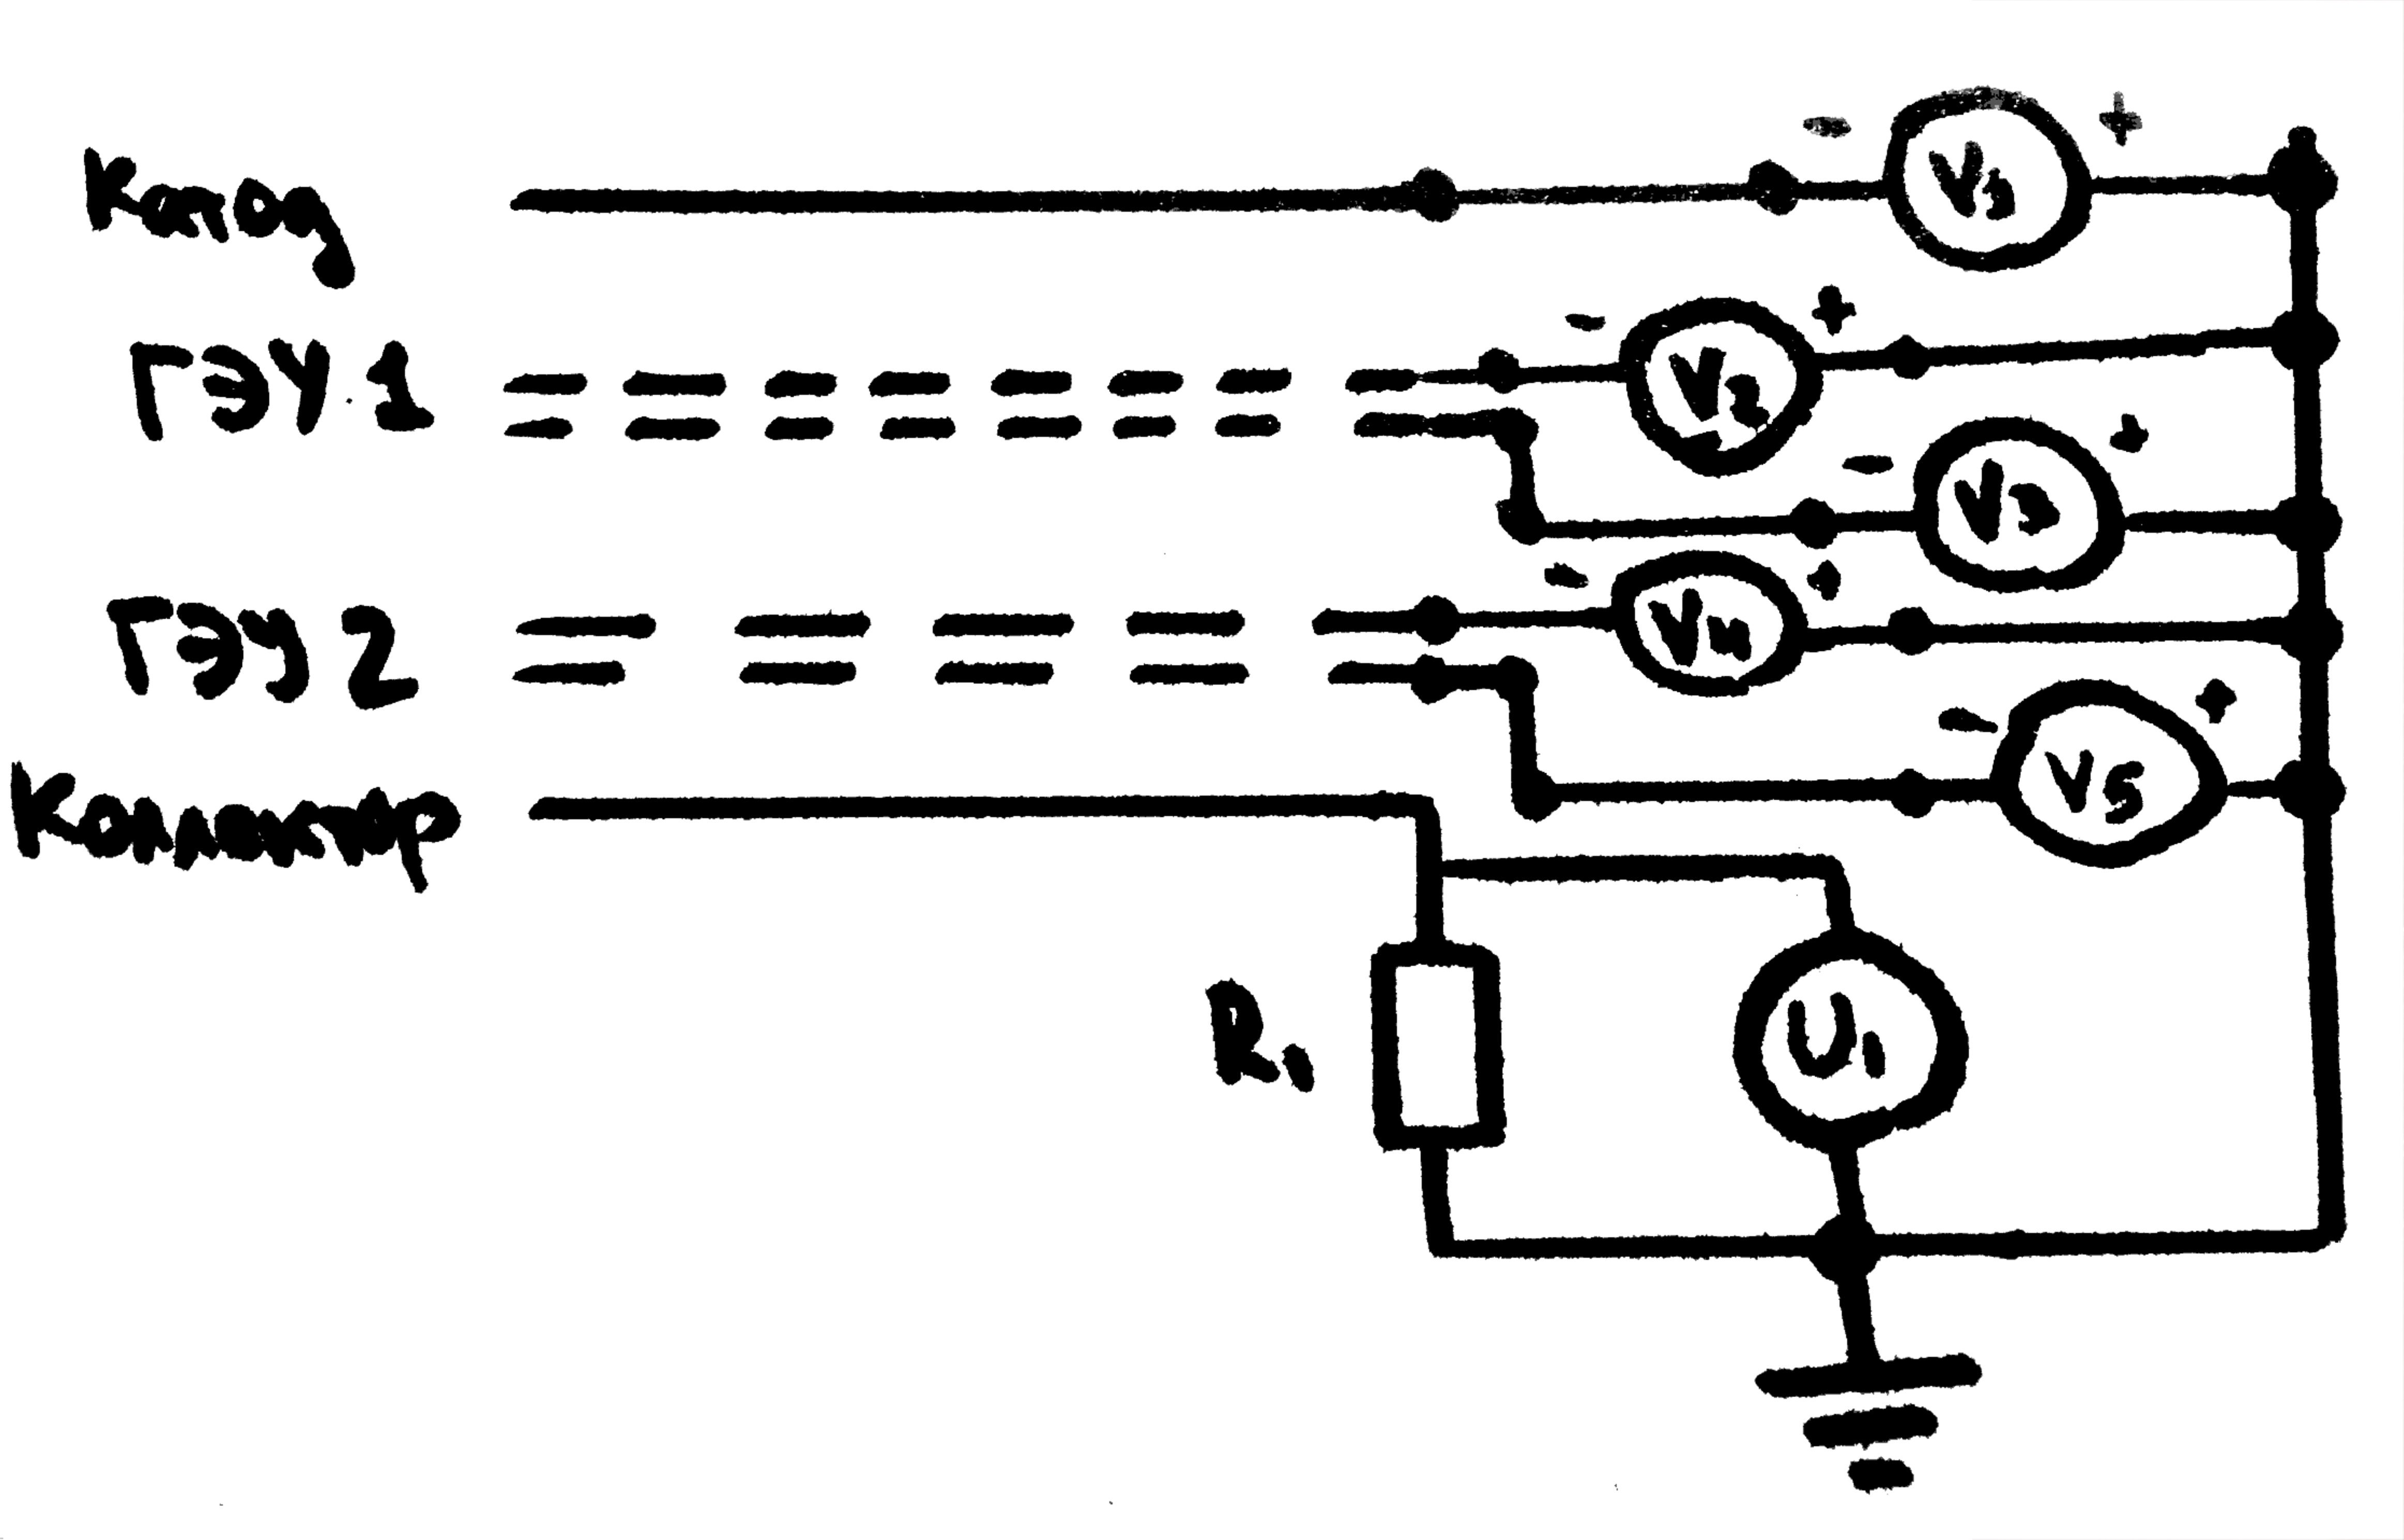
\includegraphics[width = 8cm]{img/Scheme_raether_det.pdf}
		\caption{Принципиальная электрическая схема детектора для проверки предела Рейтера. (\textit{Я её перерисую в редакторе})}
		\label{el_scheme_raether}
	\end{center}
\end{figure}
\noindent
\par Принципиальную схему детектора можно видеть на Рис.\ref{el_scheme_raether}. Напряжение на каждый электрод подавалось с отдельного источника питания ($V_1-V_5$), что обеспечивало гибкую настройку системы.
Ток с электрода-коллектора протекал через резистор $R_1$, падение напряжения на котором регистрировалось вольтметром $U_1$. 
\subsection{Проведение эксперимента}
Для создания первичной ионизации в дрейфовом промежутке использовался радиоактивный изотоп $^{109}Cd$ с активностью $10^8 \text{Бк}$\textit{Уточнить или измерить}, который излучает преимущественно фотоны с энергиями $22.1~\keV~(82.6~\%)$ и $25.0~\keV~(14.7~\%)$ который помещался сверху на катодную пластину детектора. 

